\documentclass[a4paper,12pt]{article}

%\usepackage[ngerman]{babel}
\usepackage[utf8]{inputenc}
%\usepackage{listings}
%\lstset{basicstyle=\ttfamily\small}
%\usepackage{verbatim}
%\usepackage{dingbat}
\usepackage{graphics}
\usepackage[dvipsnames,usenames,table]{xcolor}
\usepackage{amsmath,amssymb}
\usepackage{exercises}
\usepackage{../../asp}
\usepackage{url}
\usepackage{hyperref}
\usepackage{tikz}

\sloppy
\DeclareFontFamily{U}{bulb}{}
\DeclareFontShape{U}{bulb}{m}{n}{<-> lightbulb10}{}
\newcommand{\lightbulb}{{\usefont{U}{bulb}{m}{n}A}}

\newcommand*\circled[1]{\hspace{0.6mm}\tikz[baseline=(char.base)]{
    \node[shape=circle,draw,fill,inner sep=0.2mm] (char) {\color{White}\footnotesize{\textsf{\textbf{#1}}}};}}

\newcommand*\ccircle[1]{\tikz[baseline={([yshift=-8pt]current bounding box.north)}]{\draw[black,fill=#1] (0,0) circle (1ex);}}

\begin{document}
\begin{PraktikumsAufgabe}{1}{(Sudoku)}
\vspace*{-4mm}
\paragraph{Problem Description.}
%
%
The task of this project is to solve a Sudoku\footnote{\texttt{http://en.wikipedia.org/wiki/Sudoku}} 
puzzle using ASP.
The goal of the game is to fill a 9x9 grid with digits so that each column, 
each row and each of the nine 3x3 sub-grids that compose the grid
contains all numbers from 1 to 9. 
In other words, the grid has to be filled with numbers from 1 to 9 so that
the same number does not appear twice in the same row, column or 
in any of the nine 3x3 subregions of the 9x9 playing board.
Initially the grid is partially filled.

\noindent
One example is shown in Figure~\ref{fig:sudoku}.
The left figure shows the initial configuration, 
and the right figure shows the same puzzle with solution numbers marked in red.

\vspace{-4mm}
\begin{figure}[h]
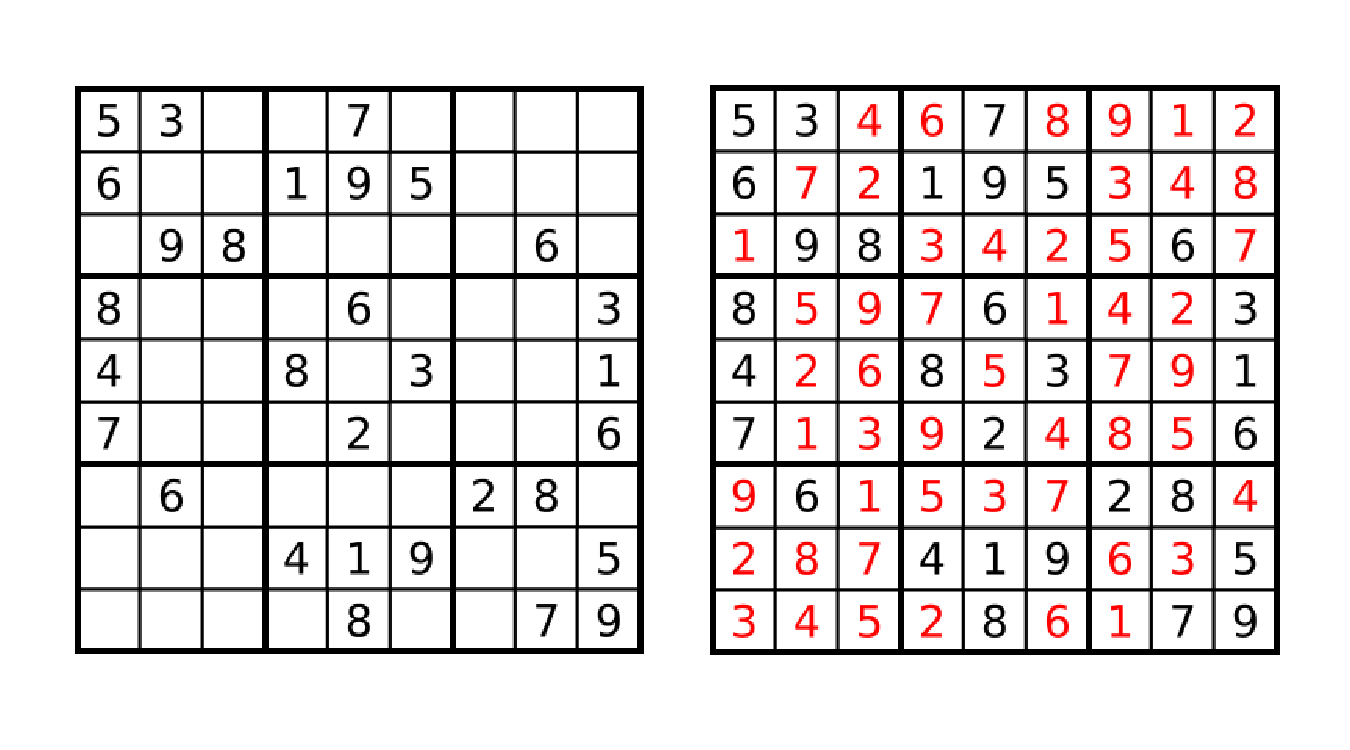
\includegraphics[width=\textwidth]{mysudoku}
\vspace{-12mm}
\caption{A sudoku and its solution.}
\label{fig:sudoku}
\end{figure}
\vspace{-4mm}


%\newpage
\paragraph{Representation in ASP.}
The initial state of the grid is represented by facts of predicate \texttt{initial/3}:
% \newpage
\vspace{-1.5mm}
\begin{verbatim}
initial(X,Y,N).   % initially cell [X,Y] contains number N 
\end{verbatim}
\vspace{-1mm}
%\newpage
For instance, the example shown in Figure~\ref{fig:sudoku} is
represented by the following facts:%
\vspace{-1.5mm}
\begin{verbatim}
initial(1,1,5). initial(1,2,3). initial(1,5,7).
initial(2,1,6). initial(2,4,1). initial(2,5,9). initial(2,6,5).
initial(3,2,9). initial(3,3,8). initial(3,8,6).
initial(4,1,8). initial(4,5,6). initial(4,9,3).
initial(5,1,4). initial(5,3,8). initial(5,6,3). initial(5,9,1).
initial(6,1,7). initial(6,5,2). initial(6,9,6).
initial(7,2,6). initial(7,7,2). initial(7,8,8).
initial(8,4,4). initial(8,5,1). initial(8,6,9). initial(8,9,5).
initial(9,5,8). initial(9,8,7). initial(9,9,9).
\end{verbatim}
\vspace{-1mm}
The solution is represented by facts of predicate \texttt{sudoku/3}:
% \newpage
\vspace{-1.5mm}
\begin{verbatim}
sudoku(X,Y,N).   % the sudoku in cell [X,Y] contains number N 
\end{verbatim}
\vspace{-1mm}
For instance, the solution of Figure~\ref{fig:sudoku} consists of the following atoms:
\vspace{-1.5mm}
\begin{verbatim}
sudoku(1,1,5) sudoku(1,2,3) ... sudoku(1,8,1) sudoku(1,9,2)
...
sudoku(9,1,3) sudoku(9,2,4) ... sudoku(9,8,7) sudoku(9,9,9)
\end{verbatim}
\vspace{-1mm}

\paragraph{Framework.}

\noindent
In the
%\href{http://www.cs.uni-potsdam.de/wv/lehre/13WS/??-Antwortprog/weaving.tar.gz}
{\texttt{sudoku.zip}}
archive at Moodle you will find five example instances.
You have to submit a file named \texttt{sudoku.lp} that contains the following line 
(and no more \texttt{\#show} statements)
so that in the output only the atoms of predicate \texttt{sudoku/3} appear:
%\footnote{These instructions hide all atoms that are not part of the solution representation.}%
\vspace{-1.5mm}
\begin{verbatim}
#show sudoku/3.
\end{verbatim}
% \begin{tabular}{l}
% \code{\#hide.}\\
% \code{\#show paint/2.}\\
% \end{tabular}
\vspace{-1mm}
% \noindent
%{\small\sf The file containing your encoding has to be called \texttt{sudoku.lp}.
%           Apart from \code{cell/3} no additional predicates must be included in the output!}

\noindent

\paragraph{Formalities.}
%
You can work on the solution alone or in groups of two people.
Different groups have to submit different solutions, 
in case of plagiarism all groups involved will fail the project.
Please submit your encoding by \textbf{Thursday 13th, 2014} via
\href{https://yeti.haiti.cs.uni-potsdam.de}{YETI}
(All group members have to create a YETI account!).
Be sure to submit your encoding in a file named \code{sudoku.lp}
containing only lowercase letters.

\noindent
We will test your encoding with the five provided instances as well as additional instances.
Your encoding has to find the correct solutions for all instances.
This will be tested automatically by YETI after you uploaded the encoding (with a slight delay).
If your solution is not correct then YETI will display an error message.
Please correct any errors that occur on your own or contact us if you get stuck.

\paragraph{Tips:}
\begin{itemize}
\item To begin with, it may be easier to represent a 4x4 sudoku and once this is done, 
      modify it to handle the 9x9 case.
\item Commands to find all stable models look as follows:%
\vspace{-1.5mm}%
\begin{verbatim}
$  gringo-4 sudoku.lp example.lp | clasp3 0
\end{verbatim}
\vspace{-1mm}
% Überlegen Sie sich, welche Bedingungen Sie zur Charakterisierung von L\"osungen
%       testen wollen und definieren Sie geeignete Pr\"adikate, die diese Tests erm\"oglichen.
% %\item Verwenden Sie die Kommandozeilenoption \texttt{--solution-recording} zur
% %      Effizienz\-steigerung bei der Berechnung aller L\"osungen, z.B.\ wie in dem folgenden Aufruf:
%
% \begin{tabular}{@{}l}%
% \texttt{[user@local \textasciitilde] clingo lights.lp test01.lp --solution-recording 0}
% \end{tabular}      
\item If you are stuck you can contact us. We will do out best to answer all your questions.
      You can send us questions and remarks via 
      \href{http://moodle.cs.uni-potsdam.de/course/view.php?id=39}{Moodle} (forum/wiki)
      or send them via mail to 
      \href{mailto:asp@lists.cs.uni-potsdam.de}{\texttt{asp@lists.cs.uni-potsdam.de}}.
\item Start as soon as possible to avoid running out of time.
      (However, if you still realize that you have problems making it before the deadline,
       please contact us instead of copying another solution).
% \item Behalten Sie Ihren Quelltext für sich.
%       Sie helfen Ihren Kommilitonen nicht, wenn Sie Ihren Quelltext weitergeben, da das Nachvollziehen eines fremden Encodings schwieriger ist als ein eigenes zu entwerfen.
\end{itemize}

\end{PraktikumsAufgabe}
\end{document}
